% put all Mike's macros in and begin document
\documentclass[pdftex]{article}
\usepackage[pdftex]{graphics}
\usepackage{subfigure}
\usepackage{hhline}
\usepackage[usenames,dvipsnames]{color}
\usepackage{colortbl}
\usepackage[screen,pdftex]{mcdlecture}
\newcommand{\bs}{\relax}
\newcommand{\es}{\newpage}
\fboxsep=.01\textwidth \fboxrule=1pt
\newsavebox{\savepar}
\newenvironment{boxit}{\begin{lrbox}{\savepar}
    \begin{minipage}[b]{0.975\textwidth}}
    {\end{minipage}\end{lrbox}\framebox{\usebox{\savepar}}}


%%%%%%%%%%%%%%%%%%%%%%%%%%%%%%%%%%%%%%%%%%%%%%%%%%%%%%%%%%
%% THE FOLLOWING ARE THINGS THAT WE MIGHT CHANGE FROM YEAR TO YEAR OR
%% VENUE TO VENUE
    \lhead{MCMC in Statistical Genetics}
    \lfoot{Dr Eric C. Anderson and Dr Matthew Stephens}
%	\lfoot{Dr Eric C. Anderson and Dr John Novembre}
%    \rfoot{UW - Summer Institute, July 2013}
%	 \rfoot{Edinburgh - European Institute, June 2012}
\rfoot{Brazil - Summer Institute, February 2014}

% on this one, be sure to update the venue and the module number
%\newcommand{\coursetitlepage}{European Institute in Statistical Genetics
%\newcommand{\coursetitlepage}{Summer Institute in Statistical Genetics
\newcommand{\coursetitlepage}{Brazilian Edition of the Summer \\Institute in Statistical Genetics

Module 9:

MCMC for Genetics}

%% Then update the schedule.  Note that I have broken that
%% out into a separate file like: schedule_table_edinburgh2012.tex
%% which is input in Overview.tex

%% Then be sure to change any time-sensitive events in the 
%% probability discussion in Matthew's first lecture.

%% And also update "structure_fun" link to my wiki to the right
%% year and venue.
%%%%%%%%%%%%%%%%%%%%%%%%%%%%%%%%%%%%%%%%%%%%%%%%%%%%%%%%%%


\begin{document}

\DeclareGraphicsExtensions{.jpg,.pdf,.png}%



%% Eric added a few things:
% some commands that Eric made for making a title while starting
% a new lecture and for making titles of new slides.
\newcommand{\newlecture}[1]{\newpage\begin{center}\section*{#1}\end{center}}
\newcommand{\newslide}[1]{\newpage\subsection*{#1: \hfil}}
 \newcommand{\Exp}{\Bbb{E}}
 \newcommand{\Var}{{\mathrm{Var}}}
 %% Some pretty etc.'s, etc...
\newcommand{\cf}{{\em cf.}}
\newcommand{\eg}{{\em e.g.},}
\newcommand{\ie}{{\em i.e.},}
\newcommand{\etal}{{\em et al.}\ }
\newcommand{\etc}{{\em etc.}}

%% some handy things for making bold math
\def\bm#1{\mathpalette\bmstyle{#1}}
\def\bmstyle#1#2{\mbox{\boldmath$#1#2$}}
\newcommand{\thh}{^\mathrm{th}}
\newcommand{\bpi}{{\pi}}
\newcommand{\mP}{\mathbf{P}}

\rhead{Session 5 - \thepage}


\definecolor{orange}{cmyk}{0,.5,1,0}
\definecolor{thetaorange}{cmyk}{.0157,.7412,.9137,0}
\definecolor{pipurple}{cmyk}{.4392,.9725,0,0}
\definecolor{wblue}{cmyk}{.9569,.9294,0,0}
\definecolor{geneblue}{cmyk}{.8,.5,0,0}
\definecolor{priorgray}{cmyk}{0,0,0,.7}

\newcommand{\squashfish}{\raisebox{-.4em}{\mbox{\includegraphics[height=1.2em]{
squash_fish.pdf}}}
}

\newcommand{\redsquashfish}{\raisebox{-.4em}{\mbox{\includegraphics[height=1.2em]{
redsquash_fish.pdf}}}
}

\newcommand{\bbfish}{\raisebox{-.8em}{\mbox{\includegraphics[height=2.1em]{
fish_bb.pdf}}}
}
\newcommand{\clearfish}{\raisebox{-.8em}{\mbox{\includegraphics[height=2.1em]{
fish_clear.pdf}}}
}
\newcommand{\rrfish}{\raisebox{-.8em}{\mbox{\includegraphics[height=2.1em]{
fish_rr.pdf}}}
}
\newcommand{\brfish}{\raisebox{-.8em}{\mbox{\includegraphics[height=2.1em]{
fish_br.pdf}}}
}
\newcommand{\rbfish}{\raisebox{-.8em}{\mbox{\includegraphics[height=2.1em]{
fish_rb.pdf}}}
}

\newcommand{\bbloc}{\raisebox{-.35em}{\mbox{\includegraphics[height=1.4em]{
loc_bb.pdf}}}
}

\newcommand{\brloc}{\raisebox{-.35em}{\mbox{\includegraphics[height=1.4em]{
loc_br.pdf}}}
}

\newcommand{\rbloc}{\raisebox{-.35em}{\mbox{\includegraphics[height=1.4em]{
loc_rb.pdf}}}
}

\newcommand{\rrloc}{\raisebox{-.35em}{\mbox{\includegraphics[height=1.4em]{
loc_rr.pdf}}}
}
\newcommand{\tc}{\textcolor}

 %
 % Declare the title, author and date as you would in regular \LaTeX.
 %
%\title{Bayesian methods for inferring population structure,
%hybridization, and migration using multilocus genetic data }
% %
%\author{\underline{Eric C. Anderson}$^\dagger$  \vspace*{1.2ex}\\
%        \textit{Department of Integrative Biology } \vspace*{-2.22ex}\\
%\\    
%       {\small University of California, Berkeley, CA, USA} }

% % This is optional
%  \date{}
%\maketitle

\newlecture{Case Study I: Inference\\ of Population Structure}
Goals of this lecture:
\begin{itemize}
\item Introduce the statistical model underlying {\sl structure} as an elaboration of a simple finite mixture model. 
\item Introduce directed graphical model notation
\item Present the two different ``flavors" of {\sl structure}'s underlying models---with and without prior population information.
\item Introduce several related methods---{\sl NewHybrids} and {\sl BayesAss+}
\end{itemize}

%\newslide{structure\hfill NewHybrids\hfill BayesAssign+}
%\noindent \textsc{Pritchard} {\em et al.} (2000)  \hfill
%\textsc{Wilson \& Rannala} (2003)  
%\begin{center}
%\includegraphics*[width=.6\textwidth]{illus/3progs.pdf}
%\end{center}
%\begin{center}
%\textsc{Anderson \& Thompson} (2002) 
%\end{center}

%\hspace*{.2in}

%\hrule

%\begin{itemize}
%\item Bayesian methods using multilocus genotypes:
%\begin{itemize}
%\item Do not require ``diagnostic" alleles
%\item Properly account for uncertainty in allele frequencies
%\item Base inference on the posterior probabilities of quantities of
%interest
%\end{itemize}
% 
%\end{itemize}






\newslide{Temporal and historical scales}

\begin{center}
\includegraphics*[width=\textwidth]{illus/mig_ice_fish.pdf}
\end{center}


% \newslide{Features of Genetic Mixture Analysis}
% \begin{itemize}
% \item Applies well to non-admixed individuals 
%\item Data Requirement:
%\begin{itemize}
%\item Multilocus genotypes of individuals sampled from the mixture
%\item Learning samples are helpful (but not necessary)
%\end{itemize}

%	\item Assumptions:
%\begin{itemize}
%\item Each individual is purely descended from one of $K$ populations
%\item Within populations there is no LD or H-WD.
%\end{itemize}

%
%\end{itemize}



\newslide{Scottish wildcat}
\begin{center}

\includegraphics[width=.8\textwidth]{illus/ScottishKitty.jpg}
\end{center}


%% ************** GENETIC MIXTURE FOIL
\newslide{Model For genetic mixture}
\vspace*{-.3in}
\begin{center}
\includegraphics*[width=.65\textwidth]{illus/mixture_cats.pdf}
\end{center}
\noindent Using a sample from the mixture the goals are to:
\vspace*{-.9ex}
\begin{enumerate}
\item Estimate the allele frequencies in Populations~0~and~1
\vspace*{-.9ex}
\item Estimate the mixing proportion $\pi$ \vspace*{-.9ex}
\item For each individual in the sample, compute the posterior
probability that it is from Population~0 or~1
\end{enumerate}


\newslide{Genetic mixture}

\begin{minipage}{.45\textwidth}
\begin{itemize}
\item $\bm{\pi}$~: the proportion of individuals from the $K$ different
sources in the mixture
\item $W_i$~: the source of individual $i$
\item $Y_{i,\ell,1}~,~Y_{i,\ell,2}$~: the two alleles at locus $\ell$ in
individual $i$ 
\item $\bm{\theta}_{\ell,1},\ldots,\bm{\theta}_{\ell,K}$ allele
frequencies at locus $\ell$ in the $K$ sources
\item $\bm{\zeta}$ and $\bm{\lambda}_\ell$ represent Bayesian priors
\end{itemize}
\end{minipage}
\hfill
\begin{minipage}{.475\textwidth}
\vfill
\hfill\includegraphics*[width=.95\textwidth]{illus/mixfishDAG.pdf}
\vfill
\end{minipage}

\newslide{DAG notation and terminology}
\begin{center}
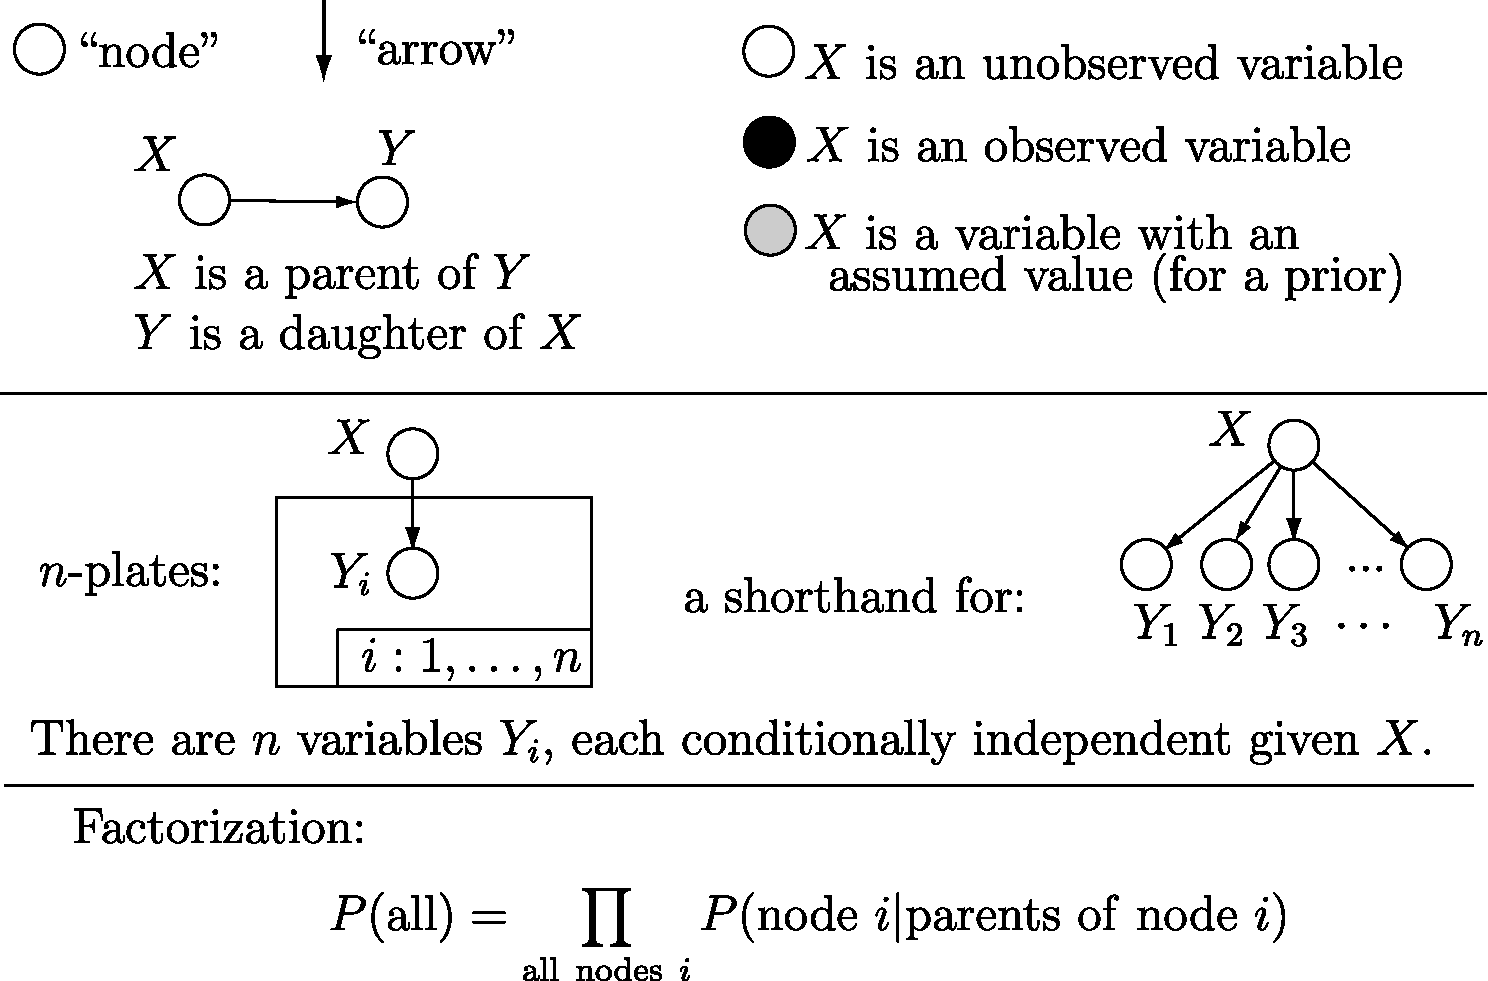
\includegraphics[width=\textwidth]{illus/dagnotat.pdf}
\end{center}



\newslide{Factorization of the joint probability density}
\begin{minipage}{.45\textwidth}
\begin{eqnarray*}
& & P(\tc{pipurple}{\bm{\pi}}|\tc{priorgray}{\bm{\zeta}})P(\tc{priorgray}{\bm{\zeta}})\times 
\mbox{}\\
%%%
& &\prod_{i=1}^M   \biggl( P(\tc{wblue}{W_i}|\tc{pipurple}{\bm{\pi}})  
\times 
\mbox{} \\
%%%
& & \prod_{\ell=1}^L
P(Y_{i,\ell,1}|\tc{wblue}{W_i},\tc{thetaorange}{\bm{\theta}_{\ell,1},
\ldots,\bm{\theta}_{\ell,K}})  \times \mbox{} \\
%%%
& & \prod_{\ell=1}^L
P(Y_{i,\ell,2}|\tc{wblue}{W_i},\tc{thetaorange}{\bm{\theta}_{\ell,1},
\ldots,\bm{\theta}_{\ell,K}}) \biggr) \times \mbox{} \\
%%%
& & 
\prod_{\ell=1}^L
P(\tc{thetaorange}{\bm{\theta}_{\ell,1},
\ldots,\bm{\theta}_{\ell,K}} | \tc{priorgray}{\bm{\lambda}_\ell})P(\tc{priorgray}{\bm{\lambda}_\ell})
\end{eqnarray*}
\vfill

\end{minipage}~~~~~~
\hfill
\begin{minipage}{.475\textwidth}
\vfill
\hfill\includegraphics*[width=.82\textwidth]{illus/mixfishDAGcolor.pdf}
\vfill
\end{minipage}



%% ************** GENETIC ADMIXTURE SCHEME
\newslide{Interbreeding complicates matters}
\vspace*{-.3in}
\begin{center}
\includegraphics*[width=.75\textwidth]{illus/admixture_cats.pdf}
\end{center}
\noindent $\bullet$ This requires a different probability model


\newslide{ Features of {\sl structure}---the admixture model (Pritchard et al. 2000) }

\begin{itemize}
\item Omnibus model---flexible and few parameters
\item Applies generically to:
\begin{itemize}
\item Hybrid zones
\item Recent gene flow
\item Population structure, cryptic or otherwise
\item Estimating the unkown number of subpopulations
\end{itemize}
\item Data Requirement:
\begin{itemize}
\item Multilocus genotypes
\item Learning samples are helpful but not necessary
\end{itemize}

\item Assumes no LD or HWD in component subpopulations
\end{itemize}




%% ************** GENETIC ADMIXTURE PROBABILITY
\newslide{The {\sl structure} model}

\begin{center}
\includegraphics*[width=\textwidth]{illus/admix_cat_flags.pdf}
\end{center}




\newslide{Genetic mixture {\em vs.} {\sl
structure}\footnote{Note that my notation departs somewhat from that in Pritchard et al.'s paper.}}
\vspace*{-.3in}
\begin{minipage}{.45\textwidth}
\mbox{}

\vspace*{.8in}

\hfill\includegraphics*[width=.95\textwidth]{illus/mixfishDAG.pdf}
\end{minipage}
\hfill
\begin{minipage}{.485\textwidth}
\vfill
\hfill\includegraphics*[width=.95\textwidth]{illus/PritchSimple.pdf}
\vfill
\end{minipage}


\newslide{Other {\sl structure} features}
There are several other bells and whistles that can be applied in {\sl structure}. 
 
A later version of structure (described in Falush et al. (2003)) includes a facility for modeling non-independence between the alleles at different loci.  This allows for linkage between markers that are near to each other on the same chromosome.

The allele frequencies in the $K$ subpopulations can also be modeled as having some correlation parameterized in terms of Wright's inbreeding parameter $F$.  Can you write down the DAG for that model?

Further elaborations include model for dominant markers and null alleles (Falush et al. 2007) and a new model for incorporating sampling location information (Hubisz et al 2009).

\newslide{Findings of \textsc{Beaumont et al.} 2001}
\begin{itemize}
\item Evidence for two distinct gene pools
\begin{itemize}
\item One inferred ``gene pool" had allele frequencies very close to
those in known domestic cats
\end{itemize}
\item Some individuals had values of $Q_i$ near 0 or 1
\item Others appeared to be quite admixed, $Q_i \approx .5$
\item Not possible to tell with {\sl structure} whether there have been
historical mixing events
\end{itemize}

\newslide{Features of {\sl
structure} (prior pop. info model)}

\begin{itemize}
\item Specialized model---more realistic in some scenarios
\item Applies specifically to:
\begin{itemize}
\item Detecting recent immigrants in populations
\end{itemize}
\item Data Requirement:
\begin{itemize}
\item Distinct subpopulation/sampling locales 
\item Multilocus genotypes
\end{itemize}
\item Assumptions:
\begin{itemize}
\item No LD or H-WD in component subpopulations
\item Number of subpopulations is known
\item Migration occurs infrequently
\item Migration rate assumed known and equal in all directions
\item Migrant ancestry limited to the last $n$ generations
\end{itemize}
\end{itemize}




%\newslide{Prior Population Information}
%
%\begin{center}
%\includegraphics*[width=.92\textwidth]{prior_popinfo_cats.pdf}
%\end{center}


\newslide{Symmetrical immigrant probability $\nu$}
\vspace*{-.4in}
\begin{center}
\includegraphics*[width=.85\textwidth]{illus/prior_popinfo_cats_nu.pdf}
\end{center}
\vspace*{-.3in}
The $i\thh$ individual is known to reside in subpopulation $S_i$.

\newslide{Immigrant ancestry with rare migration}

\begin{center}
\includegraphics*[width=.85\textwidth]{illus/immig_anc.pdf}
\end{center}
Each individual is assumed to have at most 1 migrant ancestor in the last $n$ years.

If the $i\thh$ individual has a migrant ancestor, it occured $T_i$ generations ago, and was a migrant from population $O_i$.




\newslide{{\sl structure}~~~~~~~~~~~{\em vs.}~~~~~~~~~{\sl
structure with prior pop. info}}
\vspace*{-.3in}
\begin{minipage}{.42\textwidth}
\vfill
\hfill\includegraphics*[width=.95\textwidth]{illus/PritchSimple.pdf}
\vfill
\end{minipage}
\hfill
\begin{minipage}{.475\textwidth}
\vfill
\hfill\includegraphics*[width=.95\textwidth]{illus/PritchPriorPopDuo.pdf}
\vfill
\end{minipage}

\noindent$\bullet$ Disadvantages:  must assume  $\nu$, independence
within loci, only one migrant ancestor




%\newslide{Advantages of {\sl NewHybrids}}

%\begin{itemize}
%\item Specialized scenario
%\item Applies specifically to:
%\begin{itemize}
%\item Hybridization due to recent contact
%\item Ongoing, but limited hybridization 
%\item Detecting evidence for introgression beyond the F1 stage
%\end{itemize}
%\item Data Requirement
%\begin{itemize}
%\item Multilocus genotypes
%\item Learning samples are helpful but not necessary
%\item DO NOT need sampling in separate locations
%\end{itemize}
%\item Assumptions
%\begin{itemize}
%\item No LD or H-WD within subpopulations/species
%\item Only two subpopulations/species
%\item Hybridization limited to last $n$ generations
%\end{itemize}
%\end{itemize}


%\newslide{Trout Hybridization}

%\begin{center}
%\includegraphics*[width=\textwidth]{illus/TroutPics.pdf}
%\end{center}

\newslide{Two other methods similar to {\sl structure} with prior population information}
\begin{itemize}
\item NewHybrids (Anderson and Thompson 2002)
\item BayesAss+ (Wilson and Rannala 2003)

\end{itemize}

\newslide{Features of {\sl NewHybrids}}

\begin{enumerate}
\item Does not require sampling from known, separate locations
\item Allows more than
one ``migrant ancestor" (but only 2 sources)
\item Allows non-symmetrical migration/backcrossing
\item  Dependence within loci is explicitly modeled
\begin{center}
\includegraphics*[width=.4\textwidth]{illus/parents.pdf} \hfill
\includegraphics*[width=.4\textwidth]{illus/steel_backcross.pdf}
\end{center}
\end{enumerate}


%\newslide{}
%
%\begin{itemize}
%\item Consider an F1 hybrid~~~~~~~~~~~~~~~or~~~~~~~~~~~a first
%generation backcross
%\begin{center}
%\includegraphics*[width=.45\textwidth]{parents.pdf} \hfill
%\includegraphics*[width=.45\textwidth]{steel_backcross.pdf}
%\end{center}
%\end{itemize}

\newslide{2 Generations $=$ 6 hybrid categories}

\mbox{}\hspace*{-.32in}\includegraphics*[width=.98\textwidth]
{illus/explicit_model.pdf}





\newslide{{\sl
structure with prior pop. info}~~~~~~{\em vs}.~~~~{\sl NewHybrids} }


\begin{minipage}{.5\textwidth}
\vfill
\hfill\includegraphics*[width=.95\textwidth]{illus/PritchPriorPopDuo.pdf}
\end{minipage}
\hfill
\begin{minipage}{.42\textwidth}
\vfill
\hfill\includegraphics*[width=.95\textwidth]{illus/NewHybDG.pdf}
\vfill
\end{minipage}


%\newslide{Conclusions From Trout Data}
%\begin{itemize}
%\item Strong evidence for the existence of hybrid individuals
%\item Moderate evidence for the presence of F2's
%\item However, results could be sharpened with more markers
%\end{itemize}

%

\newslide{Features of {\sl BayesAss+}}

\begin{itemize}
\item Specialized model---more realistic in some scenarios
\item Applies specifically to:
\begin{itemize}
\item Detecting recent immigrants in populations
\item Estimating separate migration rates between populations
\item Can deal with multiple locales/subpopulations
\end{itemize}
\item Data Requirement:
\begin{itemize}
\item Distinct subpopulation/sampling locales 
\item Multilocus genotypes
\end{itemize}
\item Assumptions:
\begin{itemize}
\item No LD in component subpopulations (F for H-WD)
\item Number of subpopulations is known
\item Migration occurs infrequently
\item Migrant ancestry limited to the last $n$ generations
\end{itemize}
\end{itemize}




%\newslide{North American Gray Wolf}
%\begin{center}
%\includegraphics[width=.8\textwidth]{illus/Wolf.jpg}
%\end{center}
%%\newslide{\sl
%BayesAssign+}}
%\begin{itemize}
%\item Applies specifically to:
%\begin{itemize}
%\item Recent (within 2 to 3 generations) and ongoing migration
%\end{itemize}
%\item Allows multiple subpopulations
%\item Allows separate migration rates between subpopulations
%\item Requires population information
%\end{itemize}



\newslide{{\sl BayesAss+} ~sampling scenario and model}
\begin{center}
\includegraphics*[width=.84\textwidth]{illus/wolf_demes.pdf}
\end{center}


\newslide{ {\sl
structure with prior pop. info}~~~~~~{\em vs}.~~~~{\sl BayesAss+} }
\begin{minipage}{.47\textwidth}
\vfill
\hfill\includegraphics*[width=.95\textwidth]{illus/PritchPriorPopDuo.pdf}
\end{minipage}
\hfill
\begin{minipage}{.51\textwidth}
\vfill
\hfill\includegraphics*[width=.95\textwidth]{illus/WilsonRannala.pdf}
\vfill
\end{minipage}



%\newslide{Estimated Migration Rates}
%\begin{center}
%\begin{tabular}{l|ccccccccc}
%& NR & BI & FSJ & GBL & KNP & SR & P & T/I & VI \\ \hline
%NR & .93 & .00 & .01 & .00 & .00 & .04 & .00 & .00 & .00\\
%BI & .00 & .99 & .00 & .00 & .00 & .00 & .00 & .00 & .00\\
%FSJ & .00 & .00 & .99 & .00 & .00 & .00 & .00 & .00 & .00\\
%GBL & .03 & .01 & .02 & .68 & .01 & .09 & .01 & .14 & .00\\
%KNP & .01 & .00 & .03 & .00 & .90 & .04 & .01 & .01 & .00\\
%SR & .22 & .01 & .02 & .01 & .01 & .71 & .01 & .02 & .01\\
%P & .00 & .00 & .00 & .00 & .00 & .01 & .68 & .21 & .00\\
%T/I & .03 & .01 & .01 & .00 & .00 & .23 & .00 & .72 & .00\\
%VI & .01 & .19 & .02 & .02 & .02 & .02 & .02 & .02 & .70\\
%\end{tabular}
%\end{center}

%\newslide{Details}

%\begin{itemize}
%\item Special Options in each program:
%\begin{itemize}
%\item {\sl structure}: correlated allele frequencies, linked markers
%\item {\sl  NewHybrids}: indiv's of known category, dominant markers
%(AFLP's)
%\item {\sl BayesAssign+}: Hardy-Weinberg distortions, Metropolis updates
%\end{itemize}
%\item Assessing convergence in the MCMC
%\item How many markers? 
%\begin{itemize}
%\item Rules of thumb for diagnostic markers (Boecklen and Howard 1997)
%\end{itemize}
%\item Which loci are most informative?
%\item Which populations are amenable to this kind of analysis?
%\end{itemize}

%
%\newslide{Conclusions}

%\begin{itemize}
%\item {\sl structure, NewHybrids, BayesAssign+} are all
%generalizations/extensions of a simple model for genetic mixtures
%\item ``Newer" programs represent specializations of {\sl structure} to
%handle particular scenarios:
%\begin{itemize}
%\item {\sl NewHybrids}:  recent hybridization, detecting introgression
%\item {\sl BayesAssign+}: estimating recent migration rates
%\end{itemize}
%\item If your own sampling scheme is not covered by any of these
%scenarios, further specialization is possible
%\item The utility of simulation\ldots
%\item URLs:
%\begin{description}
%\item[{\sl structure}] \texttt{http://pritch.bsd.uchicago.edu/}
%\item[{\sl NewHybrids}] {\small
%\texttt{http://ib.berkeley.edu/labs/slatkin/eriq/index.html}}
%\item[{\sl BayesAss+}]
%\texttt{http://www.rannala.org/labpages/software.html}
%\end{description}

%\end{itemize}

\newlecture{Markov chain Monte Carlo in {\sl structure}}
Goals of this lecture:
\begin{itemize}
\item Discuss component-wise Metropolis-Hastings sampling
\item Demonstrate how MCMC is carried out in the {\em structure} model
\item Introduce Gibbs sampling as a special case of Metropolis-Hastings sampling
\item Visualize MCMC in {\em structure} in real time
\end{itemize}


\newslide{Inference in the {\sl structure} model}
\begin{minipage}{.47\textwidth}
We might be interested in the posterior mean of the admixture proportions $\bm{Q}_i$ for each 
individual in the sample, \ie{}
\[
	\Exp(\bm{Q}_i|\mathbf{Y},A,\bm{\lambda})
\]
This is an expectation over the posterior distribution of $\bm{Q}_i$.

For most real scenarios, this can't be computed exactly.
\end{minipage}
\hfill
\begin{minipage}{.51\textwidth}
\vfill
\hfill\includegraphics*[width=.95\textwidth]{illus/PritchSimple2.pdf}
\vfill
\end{minipage}
\newpage

However, if we could simulate values of $\bm{\alpha}$, $\bm{Q}_i$ $\mathbf{W}$, and $\bm{\theta}$ from their distribution conditional on $\mathbf{Y}$ and the priors, then we could use that sample in Monte Carlo.  

In other words, imagine we have a sample of all the latent variables $(\bm{\alpha}, \bm{Q},\mathbf{W}, \bm{\theta})^{(1)}$, $(\bm{\alpha}, \bm{Q},\mathbf{W}, \bm{\theta})^{(2)}$, \ldots, $(\bm{\alpha}, \bm{Q},\mathbf{W}, \bm{\theta})^{(n)}$.  Then we could focus only on the simulated $\bm{Q}_i$'s, for any individuals $i$, and estimate their posterior mean by  
\[
	\Exp(\bm{Q}_i|\mathbf{Y},A,\bm{\lambda}) \approx \frac{1}{n}
	\sum_{j=1}^n \bm{Q}_i^{(j)}
\]
where $\bm{Q}_i^{(j)}$ is just one little component of the multidimensional random variable $(\bm{\alpha}, \bm{Q},\mathbf{W}, \bm{\theta})^{(j)}$ which is simulated from its conditional distriubution given the genotypic data $\mathbf{Y}$.

Simulating this ``mega-variable" can be done via a {\em component-wise} Metropolis-Hastings algorithm.

\newslide{Component-wise Metropolis-Hastings sampling I}
\begin{minipage}{.47\textwidth}
Pretend that you knew the values of all the latent variables (shaded purple here) which we will collectively call $\mathbf{X} = (\bm{\alpha}, \bm{Q},\mathbf{W}, \bm{\theta})$.
\\

 AND 
 \\
 
the value of these latent variables was randomly drawn from their conditional distribution given $\mathbf{Y}$ and the priors.
\end{minipage}
\hfill
\begin{minipage}{.51\textwidth}
\vfill
\hfill\includegraphics*[width=.95\textwidth]{illus/PritchSimple2_purp.pdf}
\vfill
\end{minipage}

\newslide{Component-wise Metropolis-Hastings sampling II}
\begin{minipage}{.47\textwidth}
Then, select a variable ($\bm{\alpha}$ here), and update it using the Metropolis-Hastings algorithm:
\begin{enumerate}
\item propose changing it to $\bm{\alpha'}$
\item accept or reject the proposal according to the M-H ratio 
\end{enumerate}
We know by the properties of the M-H algorithm, that the new state of all the variables $\mathbf{X'}$ can also be considered a random draw from $P(\mathbf{X}|\mathbf{Y},\bm{\lambda},A)$. 
\end{minipage}
\hfill
\begin{minipage}{.51\textwidth}
\vfill
\hfill\includegraphics*[width=.95\textwidth]{illus/PritchSimple2_purpprime.pdf}
\vfill
\end{minipage}
\newpage
Performing this process repeatedly, focusing on all the different components of $\mathbf{X}$ in series or in random order will lead to series of states $\mathbf{X}$ that form a Markov chain $\mathbf{X}^{(0)}, \mathbf{X}^{(1)}, \mathbf{X}^{(2)},\ldots$ and those values can be used to approximate any expectations of interest.

\vspace*{-.3in}
\subsection*{A happy consequence of the factorization:}
The $P(\mathbf{X'}|\mathbf{Y},\bm{\lambda},A)/P(\mathbf{X}|\mathbf{Y},\bm{\lambda},A)$ term in the Hastings ratio mostly cancels out.  For example, when $\mathbf{X'}$ involves an altered state of $\bm{\alpha}$:
\addtolength{\jot}{2ex}
{\small
\begin{eqnarray*}
	\frac{P(\mathbf{X'}|\mathbf{Y},\bm{\lambda},A)}{P(\mathbf{X}|\mathbf{Y},\bm{\lambda},A)} & = & 
	\frac{P(\bm{\alpha'}|A)}{P(\bm{\alpha}|A)}\cdot
	\frac{\prod_{i=1}^M P(Q_i|\bm{\alpha'})\prod_{\ell=1}^L P(W_{i,\ell,1},W_{i,\ell,2}|Q_i)\cdots}
	{\prod_{i=1}^M P(Q_i|\bm{\alpha})\prod_{\ell=1}^L P(W_{i,\ell,1},W_{i,\ell,2}|Q_i)\cdots}\\
	& = & \frac{P(\bm{\alpha'}|A)}{P(\bm{\alpha}|A)}\cdot
	\frac{\prod_{i=1}^M P(Q_i|\bm{\alpha'})}
	{\prod_{i=1}^M P(Q_i|\bm{\alpha})}
\end{eqnarray*}
}
Thus, only a portion of the complete-data, joint distribution must be considered for each update. 

\newslide{The details for an update of $\bm{\alpha}$}
The conditional distributions with $K$ subpopulations are as follows:
\begin{eqnarray*}
\alpha_k &\sim& \mathrm{Uniform}(0,A)~~,~~\mathrm{indep.~for~each~}k=1,\ldots,K  \\ 
Q_i | \bm{\alpha} &\sim& \mathrm{Dirichlet}(\bm{\alpha})
\end{eqnarray*}
New values are proposed for a single component $k$ of $\bm{\alpha}$ from a normal distribution with variance $\sigma^2$ centered at the current value $\alpha_k$:
\[
	q(\alpha_k'|\alpha_k) \equiv \mathrm{Normal}(\alpha_k,\sigma^2)~~\mathrm{Note:~this~is~symmetrical}~~~~~
\]
So the Hastings ratio for component $k=2$ looks like:
\[
 \prod_{i=1}^M \frac{\Gamma(\alpha_1+\alpha_2'+\cdots\alpha_K)}{\Gamma(\alpha_1+\alpha_2+\cdots\alpha_K)}
	\frac{\Gamma(\alpha_2)}{\Gamma(\alpha_2')} 
	\frac{Q_{i,2}^{\alpha_2'}}{Q_{i,2}^{\alpha_2}}
\]

\newslide{How about updating $\bm{Q}_i$?}
\begin{minipage}{.47\textwidth}
$Q_i$, the admixture proportion for individual $i$ is updated by a special kind of componentwise M-H algorithm called ``Gibbs Sampling."\\


Gibbs sampling (Geman and Geman 1984) is Metropolis-Hastings sampling in which the proposal distribution is the {\em full conditional} distribution of the variable being updated.  \\


The full conditional distribution is the distribution conditional on all variables that are not being changed in the update.
\end{minipage}
\hfill
\begin{minipage}{.51\textwidth}
\vfill
\hfill\includegraphics*[width=.95\textwidth]{illus/PritchSimple2_purpQprime.pdf}
\vfill
\end{minipage}

\newslide{First, focus only on the relevant variables}
\begin{minipage}{.47\textwidth}
The factorization of the joint distribution, and the conditional independencies thereof, again ensure that we only have to worry about variables in a neighborhood around $\bm{Q}_i$\\

Also, we can focus on the $\bm{Q}_i$ for a single individual $i$ at a time, rather than dealing with all $M$ individuals at once.  \\


The relevant variables appear in the pruned graph to the right.
\end{minipage}
\hfill
\begin{minipage}{.51\textwidth}
\vfill
\begin{center}
\hfill\includegraphics*[width=.75\textwidth]{illus/PritchSimple2_purpQprune.pdf}
\end{center}
\vfill
\end{minipage}

\newpage
The full conditional distribution is quite simple:
\[
P(\bm{Q}_i|\mathrm{all~other~variables}) = P(\bm{Q}|\bm{\alpha}, \bm{W})
\] 
$W_{i,\ell,1}$ is a multinomial variable (of only one trial) indicating which subpopulation the first gene copy, at the $\ell\thh$ locus in the $i\thh$ individual came from.
\begin{eqnarray*}
\bm{Q}_i | \bm{\alpha} &\sim& \mathrm{Dirichlet}(\bm{\alpha}) \\
W_{i,\ell,a} | \bm{Q}_i  &\sim&  \mathrm{Multinomial}_K(1,\bm{Q}_i)~~~~~~~\mathrm{iid}~~~\forall \ell~~\mathrm{and}~a=1,2
\end{eqnarray*}
So, it is immediately apparent that the full conditional distribution \\
$P(\bm{Q}|\bm{\alpha}, \bm{W})$ is just the posterior distribution for the cell probabilities of multinomial data---the multivariate generalization of the Beta distribution discussed in Session~1.

If $P(\bm{Q}|\bm{\alpha}, \bm{W})$ is used as the proposal distribution $q(\bm{Q'}|\bm{Q})$, then it is easy to show that the acceptance probability, computed using the Hastings ratio, is always equal to 1---a convenient feature of Gibbs sampling.  

\newslide{How about the other variables---$W$ and $\bm{\theta}$?}
The updates for these variables proceed in a similar fashion using Gibbs sampling.  


\fbox{Computer Demo}

\end{document}